\subsubsection{Boolean Logic in QUBO}\label{sec:boolean-logic-in-qubo}

One of the \textbf{strengths} of the QUBO formulation is that \hl{logical conditions can be translated into energy functions}. The \textbf{general strategy} is remarkably simple:
\begin{enumerate}
    \item \textbf{Identify} the \hl{configurations} that satisfy the desired condition.
    \item \textbf{Assign} them the \hl{lowest} possible \hl{energy}.
    \item \textbf{Assign} \hl{higher energy to all other} configurations.
    \item \textbf{Construct} a \hl{quadratic function} that reproduces those energy values.
\end{enumerate}
The \textbf{minimum of the resulting} energy function will then correspond exactly to the \textbf{solutions we want}.

\highspace
\begin{flushleft}
    \textcolor{Green3}{\faIcon{tools} \textbf{Example: XOR}}
\end{flushleft}
Let's see how this works in practice with a simple example: the \textbf{logical XOR} of two binary variables $x_1$ and $x_2$. The XOR condition is satisfied only when exactly one of $x_1$ and $x_2$ is 1: $a \ne b$. The truth table for XOR is:

\begin{table}[!htp]
    \centering
    \begin{tabular}{@{} c c | c @{}}
        \toprule
        $x_1$ & $x_2$ & XOR($x_1$, $x_2$) \\
        \midrule
        0 & 0 & 0 \\
        0 & 1 & 1 \\
        1 & 0 & 1 \\
        1 & 1 & 0 \\
        \bottomrule
    \end{tabular}
\end{table}

\noindent
The goal is to find the assignments that make the boolean function true.

\highspace
\textcolor{Green3}{\faIcon{link} \textbf{From Logic to Energy.}} Instead of directly solving the logical expression, we assign energies to each configuration. A natural choice is:
\begin{itemize}
    \item \textbf{Energy 0} for the \textbf{desired} solutions (those that satisfy the XOR condition): $(0,1)$ and $(1,0)$.
    \item \textbf{Energy 1} for the \textbf{undesired} solutions (those that do not satisfy the XOR condition): $(0,0)$ and $(1,1)$.
\end{itemize}
This gives us the following energy landscape:

\begin{table}[!htp]
    \centering
    \begin{tabular}{@{} c c | c c @{}}
        \toprule
        $x_1$ & $x_2$ & XOR & Energy \\
        \midrule
        0 & 0 & 0 & 1 \\
        0 & 1 & 1 & 0 \\
        1 & 0 & 1 & 0 \\
        1 & 1 & 0 & 1 \\
        \bottomrule
    \end{tabular}
\end{table}

\noindent
Now the optimization problem is equivalent to finding the configurations with minimum energy.

\newpage

\noindent
\textcolor{Green3}{\faIcon{tools} \textbf{Constructing the Energy Function.}} We now need to find a quadratic function $E(a, b)$ that reproduces the energy values of the table. For this simple case, we can build it incrementally:
\begin{enumerate}
    \item The configuration $(a,b) = (0,0)$ must have energy 1. So a constant temr $E = 1$ is a good starting point. However, all four configurations would then have energy 1, so additional terms are required.
    \item Next, notice that the configurations $(0,1)$ and $(1,0)$ should have energy 0. Subtracting $a$ and $b$ lowers the energy whenever one of the variables becomes 1:
    \begin{equation*}
        E(a, b) = 1 - a - b
    \end{equation*}
    But now the configuration $(1,1)$ has energy $-1$, which is too low.
    \item To fix last configuration, we add a quadratic term $2ab$ that increases the energy when both variables are 1:
    \begin{equation*}
        E(a, b) = 1 - a - b + 2ab
    \end{equation*}
    Now the energy function correctly assigns energy 0 to the desired configurations and energy 1 to the undesired ones:
    \begin{table}[!htp]
        \centering
        \begin{tabular}{@{} c c | c @{}}
            \toprule
            $x_1$ & $x_2$ & $E(x_1, x_2)$ \\
            \midrule
            0 & 0 & 1 - 0 - 0 + 2(0)(0) = 1 \\
            0 & 1 & 1 - 0 - 1 + 2(0)(1) = 0 \\
            1 & 0 & 1 - 1 - 0 + 2(1)(0) = 0 \\
            1 & 1 & 1 - 1 - 1 + 2(1)(1) = 1 \\
            \bottomrule
        \end{tabular}
    \end{table}
\end{enumerate}
Therefore, the logical problem of finding the XOR of two binary variables has been transformed into an optimization problem of minimizing the energy function:
\begin{equation*}
    E(a, b) = 1 - a - b + 2ab
\end{equation*}
The minimum energy configurations correspond exactly to the solutions of the original logical problem.

\highspace
\textcolor{Red2}{\faIcon{exclamation-triangle} \textbf{Equivalence of Formulations.}} \hl{In QUBO, the absolute value of the energy is usually irrelevant. What matters is where the minima are located.} In other words, once we have a function that correctly identifies the desired configurations as minima, \emph{\textbf{is the energy function unique?}} The answer is \textbf{no}. Different energy functions may represent the same optimization problem, provided that they preserve the same ground states.

\highspace
In this example, the formulation could be modified by adding or subtracting a constant without changing the location of the minima. For instance, we could add a constant term $-1$ to the energy function:
\begin{equation*}
    E'(a, b) = E(a, b) - 1 = (1 - a - b + 2ab) - 1 = - a - b + 2ab
\end{equation*}
Evaluating the new function:
\begin{table}[!htp]
    \centering
    \begin{tabular}{@{} c c | c @{}}
        \toprule
        $a$ & $b$ & $E'(a, b)$ \\
        \midrule
        0 & 0 & 0 \\
        0 & 1 & -1 \\
        1 & 0 & -1 \\
        1 & 1 & 0 \\
        \bottomrule
    \end{tabular}
\end{table}

\noindent
These two formulations are equivalent in terms of optimization, since they have the same minima. The choice between them is a matter of convenience and does not affect the solution of the problem. More generally, \textbf{two QUBO formulations} are considered \textbf{equivalent} if they \textbf{preserve the same ground states}, even when their energy values differ.

\highspace
This flexibility is extremely useful when constructing QUBO models. A modeler is free to choose the energy function that is easiest to derive, combine with constraints, or implement, as long as the desired solutions remain the ground states.

\highspace
\begin{flushleft}
    \textcolor{Green3}{\faIcon{tools} \textbf{Visualizing the Energy Landscape}}
\end{flushleft}
The \textbf{energy values associated with the four possible assignments can be visualized as a discrete energy landscape}. Each point corresponds to one configuration of the binary variables, while the vertical axis represents the energy assigned by the QUBO function.

\begin{figure}[!htp]
    \centering
    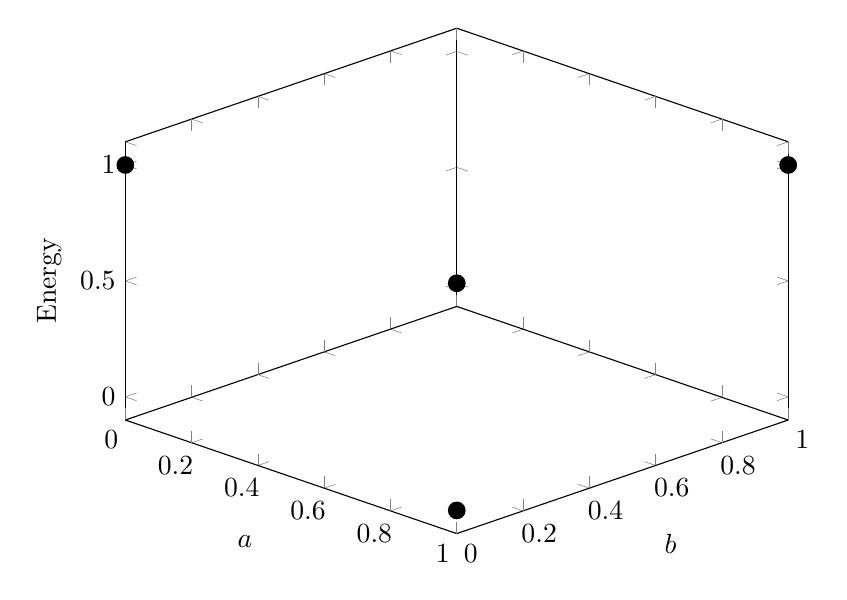
\begin{tikzpicture}
    \begin{axis}[
        view={45}{30},
        xlabel={$a$},
        ylabel={$b$},
        zlabel={Energy},
        width=10cm,
        height=8cm,
    ]
    \addplot3[
        only marks,
        mark=*,
        mark size=3pt,
    ]
    coordinates {
        (0,0,1)
        (0,1,0)
        (1,0,0)
        (1,1,1)
    };
    \end{axis}
    \end{tikzpicture}
    \caption{Discrete energy landscape of the QUBO formulation for the boolean function $a \neq b$. The ground states correspond to the minimum-energy configurations $(0,1)$ and $(1,0)$.}
\end{figure}